\documentclass[tikz, border=3mm]{standalone}
\usepackage{tikz}
\usetikzlibrary{arrows.meta, decorations.markings, angles, quotes, calc}

\begin{document}
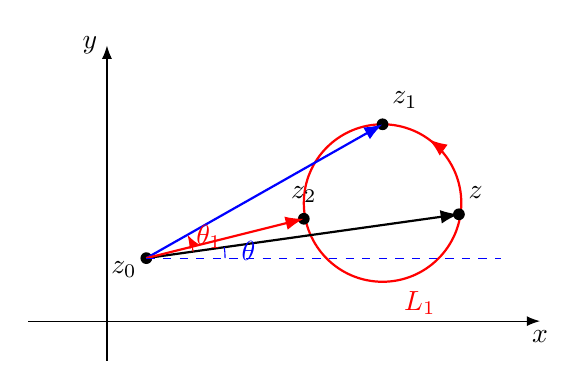
\begin{tikzpicture}[
    >=Latex, % Set default arrow tip style
    dot/.style={fill=black, circle, inner sep=1.5pt} % Style for points
]

% Axes
\draw[->] (-1, 0) -- (5.5, 0) node[below] {$x$};
\draw[->] (0, -0.5) -- (0, 3.5) node[left] {$y$};

% Define coordinates (adjusted to better match the image)
\coordinate (z0) at (0.5, 0.8);
\coordinate (z1) at (3.5, 2.5); % Point on circle
\coordinate (z)  at (4.47, 1.3569); % Point on circle (approximate)
\coordinate (z2) at (2.5, 1.3); % Intermediate point
\coordinate (c1) at (3.5, 1.5); % Estimated center of circle L1

% Draw the circle L1 using the calculated radius directly from let..in
\path let \p1=($(z1)-(c1)$), \n1={veclen(\x1,\y1)} in % \n1 is the radius in points (pt)
    % Draw the circle using \n1 directly (it's already a dimension)
    [draw=red, thick, % Move draw options here
     postaction={decorate, decoration={markings, mark=at position 0.15 with {\arrow{>}}}}
    ] (c1) circle (\n1) % Use \n1 directly
    % Position the label using \n1
    node[red, below right] at (3.64393,0.51041) {$L_1$}; % Use \n1 in polar coord
    
%\node[red,above right] ((3.5,2.5)) {$L_1$}
 %   \node[red, above right] at (-0.2, -1) {$-1$};

%\node[red, below right] at (3.64393,0.51041) {$L_1$};

% Draw points
\node[dot, label={[below left]$z_0$}] at (z0) {};
\node[dot, label={[above right]$z$}] at (z) {}; % Note: z might not be exactly on the circle now
\node[dot, label={[above right]$z_1$}] at (z1) {};
\node[dot, label={[above]$z_2$}] at (z2) {};

% Draw vectors from z0
\draw[->, thick, blue] (z0) -- (z1);
\draw[->, thick] (z0) -- (z);
\draw[->, thick, red] (z0) -- (z2); % Make vector to z2 red to match angle theta1

% Draw dashed horizontal line from z0
\coordinate (z0_horz_end) at ($(z0)+(4.5,0)$); % Point far to the right of z0
\draw[dashed, blue] (z0) -- (z0_horz_end);

% Draw angles using angles library
% Angle theta
\pic [draw, angle radius=1.0cm, "$\theta$", blue, angle eccentricity=1.3] {angle = z0_horz_end--z0--z};
% Angle theta_1 (between z0->z2 and z0->z)
\pic [draw, ->, angle radius=0.6cm, "$\theta_1$", red, angle eccentricity=1.4] {angle = z--z0--z1};

\end{tikzpicture}
\end{document}